\documentclass[tikz, border=8pt]{standalone}
\usepackage{xcolor}
\usetikzlibrary{arrows.meta, positioning, shapes.geometric, calc}
% ============================================================
% Shared style definitions for the DarwinsRNAHunt methods figures.
% \input this file from each diagram's preamble (after \usepackage{xcolor}
% and \usetikzlibrary{...}) so colours/styles stay consistent everywhere.
%
% Visual grammar used throughout:
%   - white box, single border   = external / raw resource
%   - white box, double border   = curated data artifact (output of a section)
%   - coloured box, single border = an internal processing step
%   - coloured/white, dashed border = Snakemake checkpoint (dynamic re-evaluation)
%   - white box, short-dashed border = static external file (not produced by the pipeline)
% ============================================================

% ---------- category colours (ColorBrewer Set3-style) ----------
\definecolor{catDefine}{HTML}{FFFFFF}
\definecolor{catSelect}{HTML}{FFFFFF}
\definecolor{catAcquire}{HTML}{FFFFFF}
\definecolor{catLocalize}{HTML}{FFFFFF}
\definecolor{catExtract}{HTML}{FFFFFF}
\definecolor{catCombine}{HTML}{FFFFFF}
\definecolor{catCluster}{HTML}{FFFFFF}
\definecolor{catModel}{HTML}{FFFFFF}
\definecolor{catValidate}{HTML}{FFFFFF}
\definecolor{catReport}{HTML}{FFFFFF}

% ---------- Kea Palette (defined for optional future restyling; unused for now) ----------
\definecolor{keaGreen}{HTML}{6C803A}
\definecolor{darkBrown}{HTML}{7B5C34}
\definecolor{lightBrown}{HTML}{AB7C47}
\definecolor{keaYellow}{HTML}{CCAE42}
\definecolor{keaOrange}{HTML}{D73202}
\definecolor{charcoal}{HTML}{272318}
\definecolor{lightGrey}{HTML}{D3CDBF}

\tikzset{
    font=\fontsize{7}{8}\selectfont,
    >={Latex[length=2mm,width=1.4mm]},
    every path/.style={thick},
    % internal processing step
    stage/.style={rectangle, rounded corners=2pt, draw=black, thin,
        minimum height=1.05cm, text width=3.6cm, align=center, inner sep=3pt},
    % external / raw resource (input)
    res/.style={rectangle, rounded corners=2pt, draw=black, thin, fill=white,
        minimum height=1cm, text width=4.2cm, align=center, inner sep=3pt},
    % static external file, not produced by this pipeline
    ext/.style={rectangle, rounded corners=2pt, draw=black!55, dash pattern=on 2.2pt off 1.6pt,
        thin, minimum height=0.85cm, text width=3.1cm, align=center, fill=white,
        font=\fontsize{6.3}{7.3}\selectfont, inner sep=2.5pt},
    % Snakemake checkpoint modifier (combine with stage/res)
    ckpt/.style={dashed, line width=0.9pt},
    % deliverable / output-artifact modifier: crosses a section boundary
    deliver/.style={double, double distance=1.2pt, line width=0.85pt},
    lbl/.style={font=\fontsize{8.5}{9.5}\bfseries\selectfont},
    sublbl/.style={font=\fontsize{7}{8}\itshape\selectfont},
    node distance=0.55cm and 2.6cm
}

\tikzset{edgelab/.style={font=\fontsize{6.5}{7.5}\selectfont\itshape, inner sep=2pt, align=center}}

\begin{document}
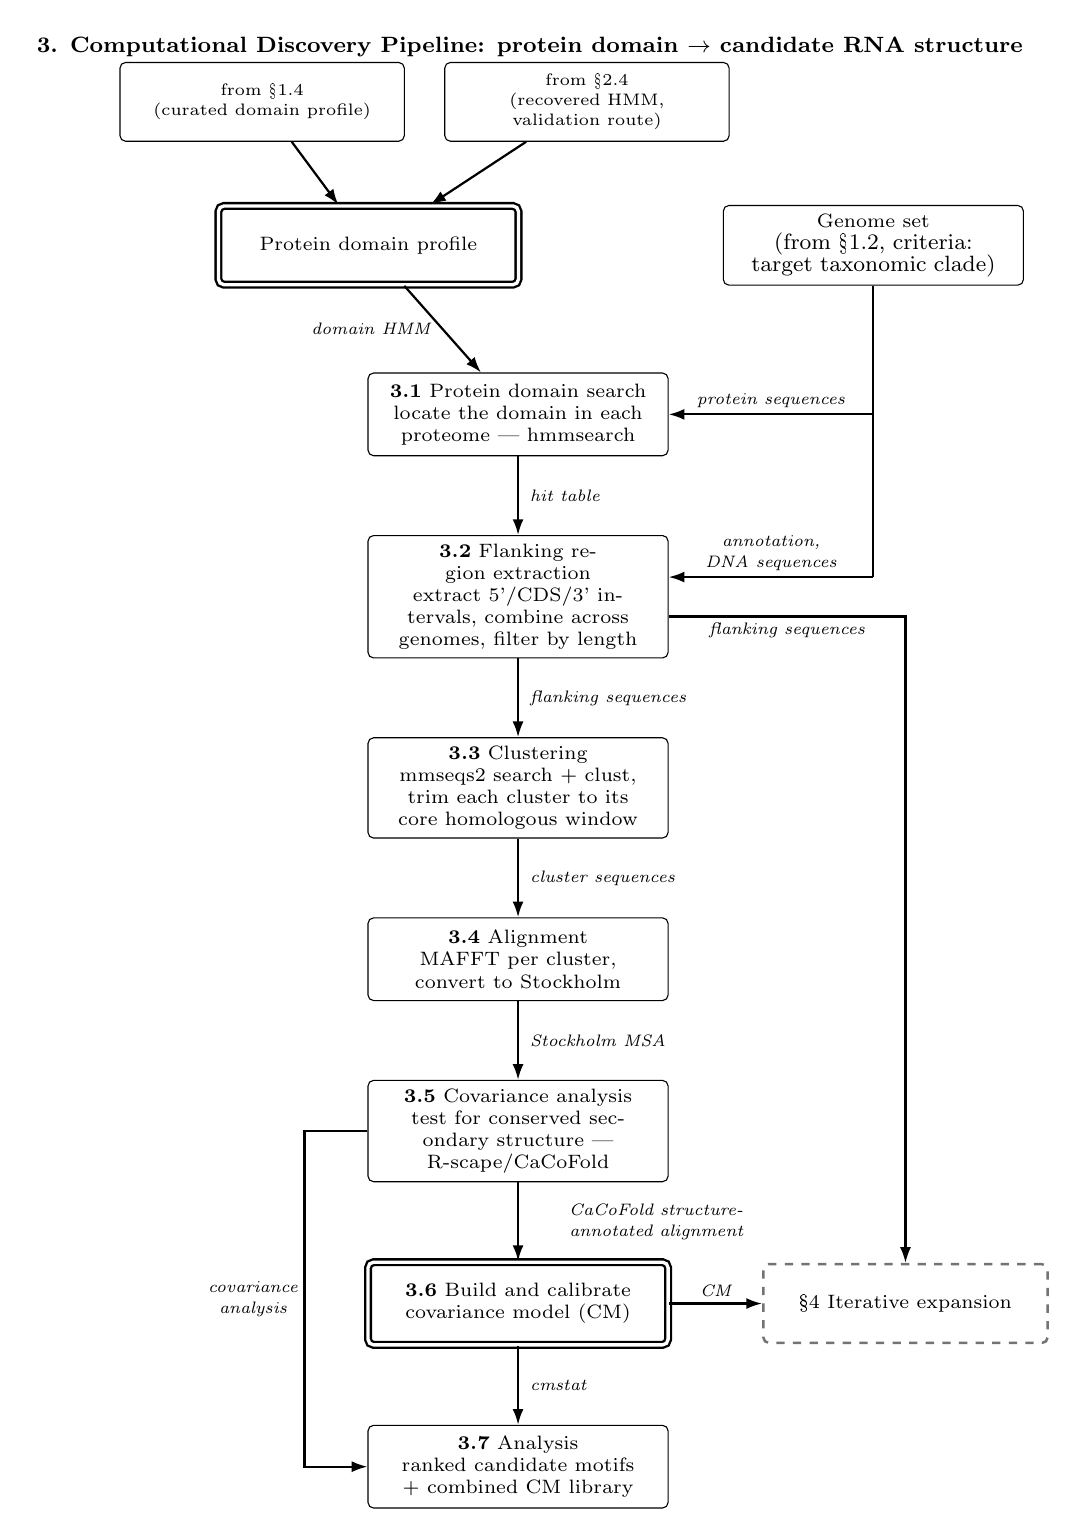
\begin{tikzpicture}

\node[lbl] (title) at (2.1,1.6) {3. Computational Discovery Pipeline: protein domain $\rightarrow$ candidate RNA structure};

% ---------------- dual-source protein input ----------------
\node[res, text width=3.4cm, font=\fontsize{6.3}{7.3}\selectfont] (src1) at (-1.3,0.9) {from \S1.4\\(curated domain profile)};
\node[res, text width=3.4cm, font=\fontsize{6.3}{7.3}\selectfont, right=0.5cm of src1] (src2) {from \S2.4\\(recovered HMM, validation route)};
\node[res, deliver, fill=catDefine!25, below=0.8cm of src1, xshift=1.35cm, text width=3.6cm] (in_domain) {Protein domain profile};
\draw[->] (src1) -- (in_domain);
\draw[->] (src2) -- (in_domain);

% ---------------- pipeline chain ----------------
\node[stage, fill=catLocalize!70, below=1.1cm of in_domain, xshift=1.9cm] (s31)
    {\textbf{3.1} Protein domain search\\locate the domain in each proteome --- hmmsearch};
\node[stage, fill=catExtract!85, below=1.0cm of s31] (s32)
    {\textbf{3.2} Flanking region extraction\\extract 5'/CDS/3' intervals, combine across genomes, filter by length};
\node[stage, fill=catCluster!55, below=1.0cm of s32] (s33)
    {\textbf{3.3} Clustering\\mmseqs2 search + clust, trim each cluster to its core homologous window};
\node[stage, fill=catModel!65, below=1.0cm of s33] (s34)
    {\textbf{3.4} Alignment\\MAFFT per cluster, convert to Stockholm};
\node[stage, fill=catValidate!55, below=1.0cm of s34] (s35)
    {\textbf{3.5} Covariance analysis\\test for conserved secondary structure --- R-scape/CaCoFold};
\node[stage, deliver, fill=catModel!65, below=1.0cm of s35] (s36)
    {\textbf{3.6} Build and calibrate covariance model (CM)};
\node[stage, fill=catReport!75, below=1.0cm of s36] (s37)
    {\textbf{3.7} Analysis\\ranked candidate motifs + combined CM library};

% ---------------- genome set: level with domain profile, right of the chain ----------------
\node[res, text width=3.6cm] (in_genomes) at ($(s31.east |- in_domain)+(2.6,0)$)
    {Genome set\\\footnotesize(from \S1.2, criteria: target taxonomic clade)};

% ---------------- section 4 stub: further right, level with 3.6 ----------------
\node[res, ckpt, draw=black!55, text width=3.4cm] (s4stub) at ($(s36.east)+(3,0)$) {\S4 Iterative expansion};

% ---------------- domain profile -> 3.1 ----------------
\draw[->] (in_domain) -- (s31) node[edgelab, midway, left=2pt] {domain HMM};

% ---------------- genome set trunk: one vertical, two branches ----------------
\coordinate (trunk31) at (in_genomes.south |- s31.east);
\coordinate (trunk32) at ($(in_genomes.south |- s32.east)+(0,0.25)$);
\draw (in_genomes.south) -- (trunk32);
\draw[->] (trunk31) -- (s31.east)
    node[edgelab, midway, above] {protein sequences};
\draw[->] (trunk32) -- ([yshift=0.25cm]s32.east)
    node[edgelab, midway, above] {annotation,\\DNA sequences};

% ---------------- main chain ----------------
\draw[->] (s31) -- (s32) node[edgelab, midway, right=2pt] {hit table};
\draw[->] (s32) -- (s33) node[edgelab, midway, right=2pt] {flanking sequences};
\draw[->] (s33) -- (s34) node[edgelab, midway, right=2pt] {cluster sequences};
\draw[->] (s34) -- (s35) node[edgelab, midway, right=2pt] {Stockholm MSA};
\draw[->] (s35) -- (s36) node[edgelab, midway, right=2pt, text width=3.2cm]
    {CaCoFold structure-annotated alignment};
\draw[->] (s36) -- (s37) node[edgelab, midway, right=2pt] {cmstat};

% ---------------- 3.5 -> 3.7 (left-hand route) ----------------
\coordinate (lx) at ($(s35.west)+(-0.8,0)$);
\draw[->] (s35.west) -- (lx) -- (lx |- s37.west) -- (s37.west);
\node[edgelab, anchor=east] at ($(lx)!0.5!(lx |- s37.west)$) {covariance\\analysis};

% ---------------- outputs to section 4 ----------------
\draw[->] (s36) -- (s4stub) node[edgelab, midway, above] {CM};

\coordinate (ex) at ($(s4stub.north |- s32.east)+(0,-0.25)$);
\draw[->] ([yshift=-0.25cm]s32.east) -- (ex) -- (s4stub.north);
\node[edgelab, above] at ($([yshift=-0.25cm]s32.east)!0.5!(ex)$) {};
\node[edgelab, below] at ($([yshift=-0.25cm]s32.east)!0.5!(ex)$) {flanking sequences};

\end{tikzpicture}
\end{document}